\documentclass{article}
\usepackage[spanish]{babel}
\usepackage[numbers,sort&compress]{natbib}
\usepackage{graphicx}

\graphicspath{ {images/} }
\usepackage{subfigure}
\usepackage{url}
\usepackage{hyperref}
\usepackage{amsmath}
\usepackage[top=15mm, bottom=40mm, left=15mm, right=15mm]{geometry}
\setlength{\parskip}{2mm}
\setlength{\parindent}{0pt}
\usepackage{listings}
\usepackage{mathrsfs}


\lstdefinestyle{mystyle}{
  numbers= left}
\lstset{style=mystyle}

\author{3175}
\title{Práctica 10: Algoritmo Genético}
\date{\today}

\begin{document}

\maketitle


\section{Introducción}

Las fuerzas entre partículas son muchas y variadas, entre las más importantes están las fuerzas electroestáticas proporcionadas por las cargas que éstas poseen la cual determina si se atraen o se repelen y la fuerza de gravedad que afecta a todo aquello que tiene una masa o inclusive una masa aparente como lo es en el caso de algunas partículas como los electrones \citep{web1}.
 
\section{Objetivo}
Determinar usando distintas reglas de asignación de valores y pesos la manera mas eficiente de reslover, el algoritmo genético con la mejor selección de valores dentro de un rango de pesos permitido.

\section{Metodología}

Usando de base el código proporcionado\citep{webelisa}, se obtiene la selección con la cantidad mas alta de la suma de valores que tengan peso permitido, por medio de la función $knapsack$, posteriormente se modifican las funciones para generar los valores de los pesos y valores: la primera con los valores asignados independientemente uno del otro, la segunda asignado independientemente pero correlacionado con el peso del objeto, esto es, entre mas pesado mas valioso, finalmente la ultima instancia es con los valores inversamente relacionados a los pesos, se verifica la distribución de los valores mediante gráficas de la figura 1.

\begin{figure}[h]
\centering
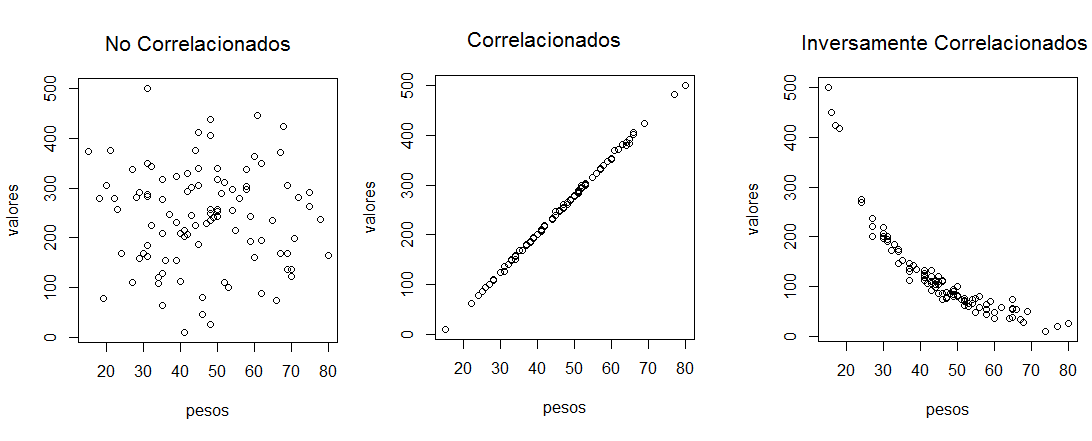
\includegraphics[width=24cm, height=7cm]{graficas.png}
\caption{Distribición de valores y pesos de los objetos}
\end{figure}

Mediante el código:

\lstinputlisting[language= R, firstline=1, lastline=48]{generadoresP10.R}


Finalmente se realiza la ejecición en paralelo del algoritmo genético y de la función $knapsack$

\lstinputlisting[language= R, firstline=109, lastline=164]{P10.R}


\section{Resultados}
Los resultados en las figuras 2,3 y 4 muestran que las asignaciones de los valores si influyen en la cantidad de tiempo que le toma resolver el algoritmo genético .


\section{Conclusiones}
Se puede determinar que los valores determinan en gran medida el tiempo que toma resolver el algoritmo genético y éste mejora contra la funcion $knapsack$ conforme  aumentan los valores.


\centering
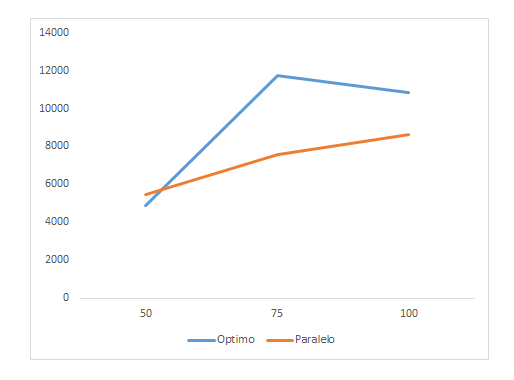
\includegraphics[width=7cm, height=7cm]{nocor.png}
\caption{Gráfica de valores no correlacionados}
\end{figure}

\begin{figure}[!ht]
\centering
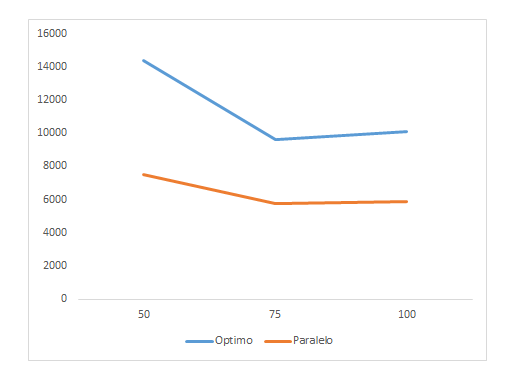
\includegraphics[width=7cm, height=7cm]{Cor.png}
\caption{Gráfica valores correlacionados}
\end{figure}

\begin{figure}[!ht]
\centering
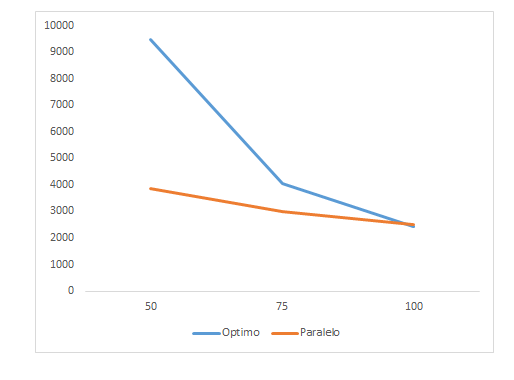
\includegraphics[width=7cm, height=7cm]{Inversamente.png}
\caption{Gráfica de valores inversamente correlacionados}
\end{figure}


\bibliographystyle{plainnat}
\bibliography{bib10}
\end{document}